\chapter{Modellizzazione f{}isica del LINAC nel TPS RayStation}
\minitoc
\textsf{In questo capitolo verranno introdotti i concetti di dosimetria di base di un acceleratore lineare. A partire da queste misure, viene costruito un modello dosimetrico del LINAC all'interno del TPS. Viene poi discussa l'accuratezza richiesta per un calcolo dosimetrico al variare della tecnica di erogazione assieme alle scelte e i metodi adottati per raggiungerla.}



\section{Dosimetria di base di un LINAC}
Le misure necessarie a costruire un modello dosimetrico di un LINAC consistono in curve di dosimetria relativa e misure puntuali di dose (assoluta e relativa).\\
Storicamente queste misurazioni vengono effettuate con detector a camera a ionizzazione\footnote{La camera a ionizzazione è un rivelatore di radiazione ionizzante a gas. \`E costituita da due elettrodi che racchiudono un certo volume di aria. Al passaggio della radiazione, l'aria viene ionizzata e libera coppie di ioni. Grazie ad un campo elettrico applicato tra i due elettrodi gli ioni migrano fino a giungere sugli elettrodi provocando un segnalo in corrente rivelabile}. Tuttavia, con l'avvento delle tecniche di radioterapia avanzata (es. intensità modulata o stereotassi) sono stati introdotti una molteplicità di detector di nuova generazione per soddisfare le esigenze di accuratezza di misura per piccoli campi di irradiazione\footnote{Un campo quadrato è ritenuto \textit{piccolo} se inferiore a $4$x$4$ cm$^2$ \cite{Das2008}.}. Nella sezione seguente verranno presentati i concetti classici di dosimetria di un LINAC propedeutici alla modellizzazione di un TPS. Ci si soffermerà dapprima alla tecnica di irradiazione denominata \textit{radioterapia conformazionale}\footnote{La radioterapia conformazionale o 3D-CRT è una tecnica di irradiazione che  fa impiego di fasci di irradiazione collimati sul target per i quali la pianificazione ed il calcolo della dose vengono effettuati su uno studio di tomografia computerizzata del paziente.}. Le problematiche relative alla dosimetria a piccoli campi e alle tecniche di irradiazione avanzata verranno discusse a seguire. 

\subsection{Dosimetria relativa}
\label{sec:dos_rel}
Per dosimetria relativa si intende tutta una serie di misure della dose non in termini assoluti (in Gray) ma in percentuale rispetto a uno o più riferimenti. In particolare le misure di dosimetria relativa necessarie alla modellizzazione di un TPS generico possono essere suddivise in tre catagorie:
\begin{itemize}
\item Curve di dose-profondità (PDD).
\item Profili di dose.
\item Output factor.
\end{itemize}
Queste misure vengono effettuate in un fantoccio cubico riempito di acqua (materiale più simile ai tessuti umani) dotato di un carrello motorizzato su cui viene montata la camera a ionizzazione che effettua le misure di dose (vedi Fig.\ref{fig:wphant}).
\begin{figure}[!t]
\centering
\includegraphics[width=.45\textwidth]{./cap2/wphant.jpg}
\includegraphics[width=.45\textwidth]{./cap2/wphant_pos.jpg}
\caption{Fantoccio per le misure di dosimetria assoluta e relativa (foto e suo posizionamento rispetto al LINAC).}
\label{fig:wphant}
\end{figure}

Le curve di dose-profondità si ottengono muovendo il detector lungo l'asse centrale del fascio (in direzione verticale) con un certo step (tipicamente 1 mm).\\
Per ogni punto, la camera a ionizzazione registra una certa dose che viene normalizzata rispetto ad una lettura di riferimento (tipicamente la lettura corrispondente alla massima dose lungo la verticale).

I profili di dose si ottengono in maniera analoga muovendo il detector in piani perpendicolari all'asse del fascio. Tipicamente vengono acquisiti profili di dose lungo due assi perpendicolari denominati \textit{inline} e \textit{crossline}\footnote{Considerando un paziente supino con la testa verso il gantry del LINAC, l'asse \textit{inline} corrisponde alla direzione testa-piedi e l'asse \textit{cross-line} alla direzione sinistra-destra.} a varie profondità.\\
\begin{figure}[!t]
\centering
\includegraphics[width=\textwidth]{./cap2/pdd_prof.png}\\
\includegraphics[width=.5\textwidth]{./cap2/of.png}
\caption{Tipici andamenti delle misure di dosimetria relativa: curva dose-profondità (PDD) (sinistra-alto); profilo di dose (destra-alto); output factor (centro).}
\label{fig:pdd_prof}
\end{figure}
Nella Fig.\ref{fig:pdd_prof} è possibile visualizzare gli andamenti tipici di una curva dose-profondità e di un profilo di dose.

Nelle curve di dose-profondità è possibile distinguere tre zone:
\begin{itemize}
\item \textit{Zona di build-up:} la prima parte ascendente della PDD in cui avvengono le prime interazioni dei fotoni nel mezzo. Gli elettroni vengono messi in moto da queste interazioni primarie e depositano energia più avanti con i processi descritti nel capitolo 1. Se non vi fossero gli elettroni di contaminazione del fascio, la dose nei primi millimetri di materiale sarebbe quasi nulla\footnote{Questo effetto è considerato un beneficio in radioterapia ed è noto anche come \textit{skin-sparing-effect.}}.
\item \textit{Massimo della PDD:} all'aumentare della profondità aumenta la produzione di particelle secondarie fino ad arrivare ad un equilibrio noto come equilibrio di particelle cariche (CPE). In queste condizioni il numero di particelle cariche uscenti da un volume è uguale al numero di particelle entranti.
\item \textit{Parte discendente della PDD:} aumentando ulteriormente la profondità di tessuto attraversato, il fascio primario decresce esponenzialmente e conseguentemente anche la dose segue questo andamento
\end{itemize}

Una distinzione simile può essere fatta per i profili di dose:
\begin{itemize}
\item \textit{Zona in-field:} la parte centrale del profilo compresa in un range di dose che va dal 100\% all'80\% rispetto alla massima dose registrata.
\item \textit{Penombra:} ai bordi del campo la dose scende rapidamente a causa della schermatura dei collimatori ed è definita come quella zona compresa tra l'80\% e il 20\% della dose massima
\item \textit{Zona out-of-field:} al di fuori delle dimensioni geometriche del campo sono presenti delle code a bassa dose che si estendono lateralmente anche al di sotto della zona schermata dai collimatori. Questa dose residua è dovuta ai processi di scatter della radiazione primaria e dei secondari. Corrisponde alla zona al di sotto del 20\% della dose massima del profilo.
\end{itemize}

Come vedremo in seguito, l'accuratezza di un calcolo dosimetrico tramite TPS viene valutata per ognuna delle zone sopra citate, con diversi livelli di tolleranza. 

Assieme alle PDD e ai profili viene anche effettuata una misura di dose puntuale al variare delle dimensioni del campo di irradiazione (\textit{output factor}). In particolare viene registrata la lettura di dose al centro del fascio ad una certa profondità (tipicamente 10 cm) e per una dimensione di campo di riferimento (10$x$10 cm$^2$). Viene quindi ripetuta la lettura al variare delle dimensioni del campo di irradiazione normalizzando il tutto alla lettura di riferimento. L'andamento che si ottiene tipicamente per un fascio di fotoni è riportato nella Fig.\ref{fig:pdd_prof}. L'output factor incrementa all'aumentare delle dimensioni del campo e ciò è dovuto principalmente ai processi di scatter che assumono più rilevanza e contribuiscono a maggiorare la lettura di dose al centro.

\subsection{Dosimetria assoluta}
\label{sec:dose_ass}
Una volta concluse le misure di dosimetria relativa, è necessario effettuare una misura di dose assoluta che permette di trasformare tutte le curve percentuali in curve di dose reale (in unità di Gray). La misurazione della dose assoluta è regolata da specifici protocolli redatti da organizzazioni internazionali come l'AAPM (America) \cite{Almond1999} e la International Atomic Energy Agency (IAEA) (Europa) \cite{Andreo2006}.\\
Per il commissioning dell'acceleratore oggetto di questa tesi è stato seguito il protocollo IAEA TRS-398 secondo cui la dose assoluta può essere ottenuta con la seguente formula:
\begin{equation}
D = M\,N_{d,w}\,k_{Q,Q_0}\,k_{TP}\,k_h\,k_{pol}\,k_{sat}
\end{equation}
dove:
\begin{description}
\item[$M:$] lettura della ionizzazione in Coulomb (effettuata con la camera a ionizzazione).
\item[$N_{d,w}:$] coefficiente di taratura della camera a ionizzazione che converte il valore in Coulomb nella dose in Gray in acqua per un fascio di riferimento (solitamente generato da una sorgente di Co-60).
\item[$k_{Q,Q_0}:$] fattore correttivo che tiene conto della diversa distribuzione energetica (qualità) di un fascio clinico generato da un LINAC rispetto al Co-60 e che dipende dalla specifica camera a ionizzazione.
\item[$k_{TP}:$] fattore correttivo che tiene conto della diversa temperatura e pressione durante la misura rispetto alle condizioni di riferimento.
\item[$k_{H}:$] fattore correttivo che tiene conto della diversa umidità durante la misura rispetto alle condizioni di riferimento.
\item[$k_{pol}:$] fattore che tiene conto della diversa lettura di carica che si ottiene con una camera a ionizzazione applicando un voltaggio positivo o negativo tra i due elettrodi.
\item[$k_{sat}:$] fattore che tiene conto degli effetti di ricombinazione delle cariche all'interno del volume di aria della camera a ionizzazione.
\end{description}
I suddetti fattori correttivi sono riportati in forma tabellare oppure si ricavano da misurazioni. Per una discussione approfondita si rimanda al protocollo \cite{Andreo2006}.

\subsection{Misure richieste per la modellizzazione del TPS RayStation}
Come già citato nelle sezioni precedenti, le misure necessarie a modellizzare un LINAC all'interno del TPS RayStation consistono in curve dose-profondità, profili di dose a varie profondità, output factor e una misura di dose assoluta per ogni qualità del fascio da modellizzare.\\
Nella Tab.\ref{tab:meas} sono indicate le dimensioni di campo per le quali è consigliato acquisire PDD, profili e gli output factor.
\begin{table}
\arrstr{1.2}
\begin{tabular}{@{}ccc@{}}
\toprule
Campi consigliati (cm$^2$) & Campi opzionali (cm$^2$) & Profondità profili (cm)\\
\midrule
2x2 & 1x1 & 1.5\\
3x3 & 4x4 & 3.0\\
5x5 & 6x6 & 5.0\\
10x10 & 7x7 & 10.0\\
15x15 & 8x8 & 15.0\\
20x20 & 9x9 & 20.0\\
30x30 & 12x12 & \\
40x40 & 25x25 & \\
\bottomrule
\end{tabular}
\caption{Misure consigliate e opzionali per le curve di PDD, profili e output factor.}
\label{tab:meas}
\end{table}
Queste misure costituiscono solo un'indicazione e possono essere estese o ridotte a seconda della tecnica di irradiazione e dell'accuratezza che si vuole raggiungere nel calcolo della dose.

\section{Accuratezza nel calcolo della dose con TPS}
\subsection{Accuratezza richiesta per la 3D-CRT}
L'accuratezza richiesta per il calcolo della dose in radioterapia conformazionale si basa su criteri stabiliti agli inizi degli anni duemila da Van Dyk et al. e Venselaar et al. \cite{Dyk1993,Venselaar2001}. Da questi due lavori pioneristici sono scaturite un certo numero di raccomandazioni da parte di organi internazionali (AAPM, ESTRO, IAEA) che hanno stabilito i limiti di accettabilità per la precisione di un calcolo di dose tramite TPS \cite{Fraass1998,Mijnheer2004,IAEA430}.\\
Il protocollo adottato per gli scopi di questa tesi è il \textit{booklet no.7} della \textit{European SocieTy for Radiotherapy \& Oncology} (ESTRO). 
\begin{figure}[!t]
\centering
\includegraphics[width=.65\textwidth]{./cap2/Accuracy_zones.png}\\\vspace{.3cm}
\includegraphics[width=\textwidth]{./cap2/Accuracy_pdd_prof.png}
\caption{In alto: suddivisione delle varie zone di interesse su cui valutare l'accuratezza del calcolo di dose con la tolleranza specifica $\delta_i$, $i\in[1,4]$. In basso: tolleranze visualizzate sulle varie zone in interesse per una PDD e un profilo di dose. I valori numerici delle tolleranze sono indicati nella Tab.\ref{tab:tol}}
\label{fig:accuracy_zones}
\end{figure}

\begin{table}
\centering
\includegraphics[width=\textwidth]{./cap2/accuracy_tol.png}
\caption{Livelli di tolleranza per le varie zone indicate nella Fig.\ref{fig:accuracy_zones} e per vari livelli di complessità del calcolo. Riprodotta da \cite{Mijnheer2004}.}
\label{tab:tol}
\end{table}
Nella radioterapia tradizionale 3D-CRT è sufficiente effettuare misure di PDD, profili e output factor per dimensioni di campo che vanno da 5$x$5 cm$^2$ a 40$x$40 cm$^2$. Per tali dimensioni di campo è possibile utilizzare detector a camera a ionizzazione senza incorrere nelle problematiche che riguardano i piccoli campi di irradiazione (< 4$x$4 cm$^2$) \cite{Das2008}. Un TPS per 3D-CRT deve riprodurre le misure effettuate con delle accuratezze variabili a seconda della regione di valutazione. Nella Fig.\ref{fig:accuracy_zones} è riportata la distinzione  nelle varie zone di interesse di un fascio di irradiazione assieme alle tolleranze applicabili ad ognuna di esse. I valori numerici sono indicati nel booklet ESTRO no.7 e sono riportati nella Tab.\ref{tab:tol}.\\
I criteri di accettabilità del calcolo vengono applicati valutando due principali quantità:

\begin{description}

\item[Differenza di dose misurata-calcolata:] questa quantità è calcolata con la formula:
\begin{equation}
\delta = 100\% \times \frac{D_{calc} - D_{meas}}{D_{N}}
\end{equation}
dove $D_{calc}$ e $D_{meas}$ rappresentano le dosi misurate e calcolate in un punto e $D_N$ rappresenta la dose di normalizzazione della differenza. Secondo le indicazioni ESTRO, $D_N$ è data dalla \textit{dose misurata locale} al punto di valutazione $D_{meas}$ nelle zone ad alta dose mentre è data dalla \textit{dose misurata a centro asse}  $D_{CAX,meas}$ nelle zone a bassa dose (es. code dei profili).\\
La valutazione in differenza di dose è adatta per le zone in cui si ha un basso gradiente di dose ($\delta D < 3\%\,$mm$^{-1}$) (es. parte discendente della PDD e parte in-field e out-field dei profili).

\item[Distanza di accordo:] questa quantità rappresenta la minima distanza tra un punto individuato dal vettore $\vec{r}_{meas}$ dove è stata misurata una certa dose e tutti i punti $\vec{r}_{calc}$ per cui la dose calcolata è  uguale a quella misurata.
\begin{equation}
DTA = \min_{\vec{r}_{calc}} \left|\vec{r}_{meas} - \vec{r}_{calc}\right|
\end{equation}
La distanza di accordo è consigliata dal protocollo ESTRO per le valutazioni di accettabilità delle zone ad alto gradiente ($\delta D > 3\%\,$mm$^{-1}$) (es. build-up delle PDD e penombre dei profili).
\end{description}

I valori di tolleranza in differenza di dose e DTA (Tab.\ref{tab:tol}) oscillano tra il 2\% - 2 mm per geometrie semplici (es. campo quadrato, fantoccio omogeneo) e il 5\% - 3 mm per i calcoli più complessi (es. dose fuori campo in condizioni di disomogeneità e asimmetria).\\
Una metodologia conveniente per eseguire una valutazione combinata dei criteri di differenza di dose e distanza di accordo è stata sviluppata da Low et al. \cite{Low1998}. Essa si basa sul dividere queste due quantità con le rispettive tolleranze e sommarle per costruire un indice adimensionale denominato \textit{$gamma$-index} (lettera greca per `c' che sta per `combined-index'):
\begin{equation}
\gamma = \min_{\vec{r}_{c}} \sqrt{\frac{|\vec{r}_{m}-\vec{r}_{c}|^2}{\Delta r}   + \frac{\left[D_{m}(\vec{r}_{m})-D_{c}(\vec{r}_{c})\right]^2}{\Delta D} }
\end{equation}
dove i pedici `$m$' e `$c$' indicano `misurato' e `calcolato' e $\Delta r$ e $\Delta D$ costituiscono le tolleranze rispettivamente per la distanza di accordo e la differenza di dose. Il criterio di accettabilità viene soddisfatto nel punto di interesse se risulta $\gamma < 1$.

Tuttavia, le raccomandazioni ESTRO sconsigliano di valutare l'accettabilità del calcolo di un profilo o PDD con un criterio puntuale bensì di utilizzare un criterio che consideri tutti i punti della curva di dose. Questo criterio è detto livello di confidenza dell'indice $\gamma$ ed è stato introdotto da Venselaar et al.\cite{Venselaar2001}:
\begin{equation}
CL(\gamma) = \bar{\gamma} + 1.5\,\sigma(\gamma)
\label{eq:clgamma}
\end{equation}
dove $\bar{\gamma}$ è la media di tutti i valori dell'indice $\gamma$ calcolati sulla curva di dose e $\sigma(\gamma)$ è la loro deviazione standard (vedi Fig.\ref{fig:gamma10x10}).
Il confronto tra una curva di dose misurata e la corrispettiva calcolata risulta in tolleranza se il livello di confidenza dell'indice $\gamma$ risulta minore di 1 ($CL(\gamma) < 1$).
\begin{figure}[!t]
\centering
\includegraphics[width=.9\textwidth]{./cap2/pdd10x10.png}
\caption{Confronto tra una PDD misurata e calcolata con il criterio del livello di confidenza dell'indice $\gamma$. Dalla distribuzione dei valori dell'indice $\gamma$ vengono calcolate la media e la deviazione standard e applicata la formula di Venselaar \eqref{eq:clgamma} per il calcolo del livello di confidenza dell'indice $\gamma$. Nel caso indicato in figura $CL(\gamma)=0.33$}
\label{fig:gamma10x10}
\end{figure}

\subsection{Accuratezza richiesta per le tecniche avanzate (IMRT e VMAT). La problematica dei piccoli campi di irradiazione}
Per tecniche `avanzate' si intendono maggiormente le tecniche ad intensità modulata (IMRT). A differenza della 3D-CRT, queste tecniche realizzano una distribuzione di dose modulata all'interno del medesimo fascio di irradiazione con il beneficio di ottenere una maggiore conformazione della dose attorno al bersaglio \cite{ICRU2010} (Fig.\ref{fig:3D_IMRT}).\\
\begin{figure}[!t]
\centering
\includegraphics[width=\textwidth]{./cap2/3D_IMRT.png}
\caption{Differenza tra fasci di irradiazione conformati (3D-CRT) e fasci erogati in tecnica ad intensità modulata (IMRT).}
\label{fig:3D_IMRT}
\end{figure}
La modulazione della dose può essere realizzata in modalità \textit{step-and-shoot} (SMLC) ossia sommando una serie di fasci caratterizzati da diverse collimazioni (segmenti) \cite{Bortfeld1994} oppure in modalità \textit{dinamica}  (DMLC) che realizza la modulazione muovendo dinamicamente il multi-leaf-collimator \cite{LING1996}. Più recentemente è stata introdotta un'ulteriore modalità detta \textit{arcoterapia volumetrica} (VMAT) che realizza una distribuzione di dose modulata collimando il fascio durante la rotazione del gantry e modificando contemporaneamente il rateo di dose \cite{Otto2008}.\\
La caratteristica che accomuna tutte queste tecniche è il largo uso di campi di piccole dimensioni (i.e. $<4x4$ cm$^2$ \cite{Das2008}). Per questo motivo, per il commissioning di un TPS dedicato alla pianificazione di trattamenti IMRT o VMAT, è necessario estendere le misure di PDD, profili e output factor ai campi piccoli ed anche rivalutare l'accuratezza tollerabile per un calcolo dosimetrico.

La dosimetria dei piccoli campi di irradiazione presenta varie criticità \cite{Das2008} tra cui:
\begin{itemize}
\item Mancanza di equilibrio di particelle cariche (CPE) laterale.
\begin{itemize}
\item[-] Questo effetto si realizza quando le dimensioni del campo sono comparabili con il range medio degli elettroni secondari. Per energie del fascio primario minori di $10\,$MV il CPE non è soddisfatto per dimensioni di campo al di sotto di $3x3\,$cm$^2$.
\end{itemize}
\item Apertura dei collimatori comparabili con la dimensioni proiettate della sorgente.
\begin{itemize}
\item[-] Questo crea un doppio effetto che consiste in una forte riduzione della dose sull'asse centrale del fascio e assieme ad una modificazione della forma del profilo (forma ogivale e allargamento della penombra) (vedi Fig.\ref{fig:small_eff})
\end{itemize}
\item Dimensioni dei detector comuni comparabili con le dimensioni del campo.
\begin{itemize}
\item[-] Ciò può portare ad un effetto di \textit{volume averaging} indicato nella Fig.\ref{fig:small_eff} che si traduce in una sottostima del massimo della dose al centro e ad una modificazione delle penombre.
\end{itemize}
\end{itemize}
\begin{figure}[!t]
\centering
\includegraphics[width=.7\textwidth]{./cap2/small_eff1.png}
\includegraphics[width=.7\textwidth]{./cap2/small_eff2.png}
\caption{In alto: la sovrapposizione delle penombre dei collimatori (legate alle dimensioni della sorgente primaria) porta ad una modificazione della forma del profilo di dose (forma ogivale e penombre allargate) assieme ad una forte riduzione della dose al centro. In basso: criticità nell'utilizzo di detector di dimensioni comparabili con la dimensione del campo.}
\label{fig:small_eff}
\end{figure}

Queste condizioni sono lontane dalle tipiche condizioni di riferimento dettate dai consolidati protocolli di dosimetria \cite{Almond1999,Andreo2006} pensati per la 3D-CRT in cui non vengono impiegati campi di piccole dimensioni (i.e. $<4x4\,$cm$^2$ \cite{Das2008}). Per minimizzare le incertezze che derivano da queste criticità sui piccoli campi, negli anni sono stati sviluppati una serie di detector di nuova generazione quali micro-camere a ionizzazione, rivelatori a semiconduttore, rivelatori a scintillazione etc., con l'intento comune di ridurre le dimensioni del volume sensibile, preservando le caratteristiche di affidabilità di un detector comunemente impiegato per 3D-CRT (linearità, indipendenza dall'energia, indipendenza dal rateo di dose\ldots).\\
Una estensiva review dei detector, delle loro problematiche e delle tecniche di misura consigliate per piccoli campi è stata recentemente pubblicata dal task group (TG) 120 dell'associazione americana dei fisici medici (AAPM) \cite{Low2011}. Sulla base dei risultati passati in rassegna dal TG-120, la comunità scientifica dell'AAPM e della IAEA è al lavoro congiuntamente per aggiornare i classici protocolli di dosimetria ed emettere delle nuove raccomandazioni che permettano una misura accurata della dose anche in presenza delle succitate criticità. In conclusione, una parte rilevante dell'accuratezza richiesta nel calcolo della dose in IMRT e VMAT è legata all'accuratezza con cui viene effettuata la dosimetria dei piccoli campi in quanto parti rilevanti della modellizzazione del TPS si basano su queste misurazioni.

Accanto all'accuratezza richiesta nell'acquisizione delle misure, vi è l'accuratezza del calcolo del dose da considerare. Le indicazioni relative all'accuratezza di un TPS per IMRT sono state studiate dal task group 119 della AAPM \cite{Ezzell2009}. Il report suggerisce di conservare ed estendere le tolleranze per 3D-CRT riportate in Tab.\ref{tab:tol} per i campi piccoli e di revisionare la formula di Venselaar \eqref{eq:clgamma}:
\begin{equation}
CL(\gamma)_{\text{IMRT}} = \bar{\gamma} + 1.96\,\sigma(\gamma)
\end{equation}
Oltre ad indicare i criteri di accettazione per le curve di dose, il TG-119 riporta anche delle tolleranze di accettabilità per una serie di test che simulano delle comuni situazioni cliniche e che sono stati presi in considerazione nelle fasi finali del commissioning del TPS. 

\section{Scelte adottate per le misure}
\subsection{PDD e Profili di dose}
Il LINAC oggetto di questa tesi è un modello Trilogy\textsuperscript{\textcopyright} prodotto dalla Varian Medical Systems. Esso è progettato per poter erogare trattamenti radioterapici in tecnica conformazionalee e ad intensità modulata (IMRT) step-and-shoot e dinamica fino ad una dimensione di campo massima $40x40\,$cm$^2$. \`E inoltre in grado di erogare trattamenti volumetrici ad arco con intensità e rateo di dose modulati (VMAT) fino ad una dimensione di campo massima $30x30\,$cm$^2$. Oltre a queste caratteristiche legate all'erogazione è inoltre capace di effettuare uno studio di tomografia computerizzata del paziente prima del trattamento in modo da verificare in tre dimensioni l'accurata collocazione sia del paziente in sé sia dei suoi organi interni, rispetto alle posizioni pianificate.

La distanza sorgente-superficie dell'acqua (SSD) è stata posta a $90\,$cm sulle basi delle raccomandazioni della ditta ed anche del report 106 dell'AAPM \cite{Das2008a} che indica $90\,$cm come la SSD più vicina alle condizioni dei trattamenti più comuni.

Seguendo poi le linee guida AAPM TG-120 citate nella sezione precedente \cite{Low2011} e tenendo conto delle raccomandazioni della ditta produttrice del TPS (Tab.\ref{tab:meas}), le scelte effettuate per le misure di PDD e profili di dose sono le seguenti:
\begin{itemize}
\item Dimensioni di campo (in cm$^2$) $5x5$, $7x7$, $10x10$, $15x15$, $20x20$, $30x30$ e $40x40$ misurate con detector a camera a ionizzazione modello CC13 prodotto dalla IBA Dosimetry (volume attivo: $0.13\,$cm$^3$).
\item Dimensioni di campo (in cm$^2$) $1x1$, $2x2$, $3x3$ e $4x4$ misurate con detector a semiconduttore (diodo) modello PFD prodotto dalla IBA Dosimtery (volume attivo: $0.09\,$mm$^3$).
\end{itemize}
Queste scelte ricalcano le raccomandazioni dei consolidati protocolli di dosimetria per quanto riguarda l'utilizzo della camera a ionizzazione per i campi al di sopra di $4x4\,$cm$^2$ mentre considerano le nuove evidenze sperimentali \cite{Das2008a,Low2011} riguardo l'utilizzo di detector di piccole dimensioni per i campi al di sotto di $5x5\,$cm$^2$. Nello specifico, in Fig.\ref{fig:pen_of}) vengono confrontate le penombre dei profili di dose misurate con vari detector tra cui quelli utilizzati nell'ambito di questo lavoro.
\begin{figure}[!t]
\centering
\includegraphics[width=.75\textwidth]{./cap2/pen_smear.png}\\
\includegraphics[width=.75\textwidth]{./cap2/OF_uncert.png}
\caption{In alto: Effetto di smussamento della penombra dei profili dovuto al volume esteso delle camere a ionizzazione confrontato con scansioni effettuate con detector di dimensioni ridotte\cite{Das2008a}. In basso: misura degli output factor a piccoli campi a seconda del detector impiegato\cite{Das2008}.}
\label{fig:pen_of}
\end{figure}
Si può notare come le camere a ionizzazione con estesi volumi sensibili ($0.6\,$cc e $0.3\,$cc) portino ad una sovrastima della penombra del profilo a causa dell'effetto di volume-averaging. L'effetto è tanto più trascurabile quanto più viene diminuita la dimensione del detector (es. micro-camera a ionizzazione con volume sensibile di $0.125\,$cc oppure detector a semiconduttore come PFD e SFD). L'accurata misura delle penombre, è di cruciale importanza in quanto vedremo che la modellizzazione delle dimensioni della sorgente primaria è tanto più accurata quanto più lo sono le misure di penombra dei campi di piccole dimensioni.

\subsection{Output factor}
Come già introdotto nella Sez.\ref{sec:dos_rel}, gli output factor (OF) costituiscono misure di punto relative e si determinano per ogni dimensione campo di cui sono state acquisite le PDD e i profili con la formula:
\begin{equation}
\label{eq:OF}
OF(XxY)=\frac{D(XxY)}{D(10x10)}
\end{equation}
dove $D(XxY)$ è la lettura di dose per un campo di dimensioni $XxY\,$cm$^2$ e $D(10x10)$ è la lettura di dose per il campo di riferimento ($10x10\,$cm$^2$). Tutte le letture di dose sono effettuate a centro asse e a $10\,$cm di profondità\footnote{In dosimetria relativa il termine `dose' è utilizzato come sinonimo di carica integrata raccolta dal rivelatore per un fissato intervallo di tempo.  Ciò non è da confondere con la `dose' in dosimetria assoluta che comporta un processo di misura più complesso (Sez.\ref{sec:dose_ass}).}.

Seguendo le indicazioni delle ditta produttrice del TPS \cite{RaySearchLaboratories2014}, gli OF sono stati misurati per ogni dimensione di campo con il medesimo detector utilizzato per le misure di PDD e profili di dose. Mentre per i campi al di sopra del $4x4\,$cm$^2$ è stata impiegata una camera a ionizzazione secondo una procedura consolidata per la 3D-CRT \cite{Andreo2006}, il rivelatore a semiconduttore PFD utilizzato per i campi piccoli può presentare delle criticità. Varie evidenze scientifiche riassunte dall'AAPM TG-120 \cite{Low2011} hanno dimostrato che la classe di dosimetri basata su semiconduttore al silicio tende a sovrastimare la lettura di dose \cite{Low2011}. Ciò è dovuto al più alto numero atomico del silicio rispetto al numero atomico medio dell'acqua che comporta un aumento dell'efficienza di rivelazione dei fotoni a bassa energia\footnote{Fotoni di bassa energia interagiscono principalmente per effetto fotoelettrico la cui probabilità di accadimento è proporzionale a $Z^3$.}. L'effetto è marcato per campi grandi (i.e. $> 4x4\,$cm$^2$) in cui i fotoni a bassa energia aumentano in percentuale. Un tipico rimedio a ciò consiste nello schermare il volume di silicio con un materiale ad alta densità (tungsteno nel caso del PFD) che assorbe i fotoni a bassa energia per compensare l'effetto di sovra-risposta. Tuttavia, sebbene si recuperi la sovra-risposta per campi grandi, il materiale ad alta densità nel detector comporta degli effetti di scatter che perturbano la lettura di dose causando una sovra-risposta per i campi piccoli \cite{Griessbach2005}.

Per poter effettuare una valutazione dell'incertezza degli OF misurati con il rivelatore a semiconduttore PFD, è stato quindi condotto uno studio che ha implicato l'utilizzo di una serie di detector di differente natura. In particolare è stato effettuato un interconfronto dei rivelatori indicati nella Tab.\ref{tab:OF_inter}.\\ I risultati di questo interconfronto sono riportati in Fig.\ref{fig:OF_res} che possono essere comparati qualitativamente con la Fig.\ref{fig:pen_of}.
\begin{table}[!t]
\centering
\arrstr{1.3}
\begin{threeparttable}
\begin{tabular}{llll}
\toprule
Nome modello & Tipo & Produttore & Volume attivo (cm$^3$)\\
\midrule
CC13 & CI\tnote{1} & IBA Dosimetry & $0.13$\\
CC01 & CI & IBA Dosimetry & $0.01$\\
Exradin A26 & CI & Standard Imaging & $0.015$ \\
Exradin W1 & SC\tnote{2} & Standard Imaging & $0.0024$ \\
PFD & Diodo SI\tnote{3} & IBA Dosimetry & $0.00009$ \\
SFD & Diodo SI & IBA Dosimetry & $0.00001$ \\
Razor & Diodo SI & IBA Dosimetry & $0.000006$ \\
\bottomrule
\end{tabular}
\begin{tablenotes}[para]
\item[1] CI: Camera a ionizzazione
\item[2] SC: Scintillatore
\item[3] SI: Semiconduttore (Silicio)
\end{tablenotes}
\end{threeparttable}
\caption{Detector utilizzati per lo studio degli output factor a piccoli campi.}
\label{tab:OF_inter}
\end{table}
\begin{figure}[!t]
\centering
\includegraphics[width=.8\textwidth]{./cap2/OF_plots/OFCC13.eps}\\
\includegraphics[width=.8\textwidth]{./cap2/OF_plots/OFSmall.eps}
\caption{Sopra: output factor misurati con la camera a ionizzazione; da notare è la normalizzazione ($OF=1$) per il campo $10x10\,$cm$^2$. Sotto: interconfronto tra vari detector nella stima degli output factor dei piccoli campi.}
\label{fig:OF_res}
\end{figure}
In esse si può notare come la misura degli OF per piccoli campi presenti un certo grado di variabilità a seconda del detector utilizzato. Le variabilità più ampie si riscontrano per i campi di dimensione $\leq 1x1\,$cm$^2$ (superiori al $5\%$, vedi Tab.\ref{tab:delta_OF}). 

\begin{table}
\centering
\arrstr{1.3}
\begin{tabular}{cllllll}
\toprule
  & \multicolumn{6}{c}{$\Delta$PFD vs.}\\
  \cmidrule{2-7}
 
Field Size (cm$\,x\,$cm$^2$) & CC13 & CC01 & A26 & W1 & SFD & Razor\\
\midrule
$1x1$ &        & $8.6\%$ & $9.6\%$ & $5.7\%$ & $8.3\%$ & $9.1\%$\\
$2x2$ & $3.2\%$ & $3.5\%$ & $2.1\%$ & $0.6\%$ & $5.4\%$ & $6.1\%$\\
$3x3$ & $1.4\%$ & $2.5\%$ & $1.2\%$ &  &      & $5.1\%$ \\
$4x4$ & $1.1\%$ & $1.9\%$ & $1.0\%$ & $-0.3\%$ & $3.8\%$ & $4.4\%$ \\
$5x5$ & $0.8\%$ & $1.2\%$ & $0.8\%$	&         & $3.1\%$ & $3.7\%$ \\
$7x7$ & $0.4\%$ & $0.8\%$ & $0.2\%$	&         &         &         \\
\bottomrule
\end{tabular}
\caption{Variabilità degli output factor misurati con i diversi detector espressi come differenza percentuale rispetto al detector scelto per le misure di commissioning (PFD della IBA Dosimetry).}
\label{tab:delta_OF}
\end{table}

Il diodo PFD, in accordo con il comportamento atteso per campi grandi \cite{Griessbach2005}, misura degli OF simili a quelli misurati con la camera a ionizzazione CC13. In particolare, per campi $\geq 5x5\,$cm$^2$ la deviazione tra il PFD e la camera CC13 risulta inferiore all'$1\%$ (Tab.\ref{tab:delta_OF}). Per campi piccoli ($\leq 4x4$cm$^2$) si nota invece una sovrastima dell'ouput factor che diventa rilevante per il campo $1x1\,$cm$^2$ ($\Delta > 5\div9\%$ ).

Parallelamente ai diodi schermati, esistono in commercio anche detector basati su silicio non schermato (i.e. SFD e Razor della IBA Dosimetry). Per questi detector l'effetto di sovrastima dell'OF a piccoli campi è ridotto, tuttavia viene amplificato quello a campi grandi. Le correnti raccomandazioni di misura degli OF \cite{Andreo2006,RaySearchLaboratories2014} stabiliscono come campo di riferimento quello di dimensioni $10x10\,$cm$^2$. La lettura di dose per questo campo, effettuata con un diodo non schermato, risulta sovrastimata per l'abbondanza dei fotoni a bassa energia \cite{Griessbach2005}. Sovrastimando la lettura di riferimento, gli OF per campi più piccoli risulteranno sottostimati. Questo effetto è visibile nella Fig.\ref{fig:OF_res} in cui risulta chiara la sistematicità della sottostima degli OF misurati con i diodi non schermati (SFD e Razor), rispetto a tutti gli altri detector.

A causa delle dimostrate criticità nella misura degli OF a piccoli campi, è stato proposto di revisionare i protocolli correnti introducendo, tra le altre cose, una correzione alla misura degli output factor che tiene conto della geometria di misura e della natura del detector utilizzato \cite{Alfonso2008}. In particolare l'Eq.\eqref{eq:OF} si aggiunge di un fattore:
\begin{equation}
OF(XxY)=\frac{D(XxY)}{D(10x10)}\times k
\end{equation}
dove il fattore $k$ dipende dalle dimensioni del campo, dalla qualità del fascio, dalla profondità di misura dell'OF etc. e serve a compensare le criticità legate alla natura del detector.\\
I fattori $k$ si calcolano con metodo Monte Carlo simulando tutto il processo di irradiazione e raccolta della ionizzazione da parte del particolare detector. Queste simulazioni sono condotte da vari gruppi di ricerca affiliati al task group n. 155 della AAPM e i risultati verranno inclusi nel report contenente le raccomandazioni per la dosimetria a piccoli campi \cite{AAPMTG155}. 

Tuttavia, al tempo di redazione di questo lavoro (Gennaio 2016), il report risulta ancora in sviluppo per cui una correzione degli OF misurati con un certo detector va valutata con cautela. Considerando le tolleranze nella Tab.\ref{tab:tol} estese anche ai campi piccoli \cite{Low2011}, si può adottare una soglia del $2\%$ sulla valutazione degli OF. Osservando la Tab.\ref{tab:delta_OF} si nota che il detector PFD fornisce valori in accordo con il detector Exradin W1 fino ad un campo di dimensioni $2x2\,$cm$^2$. Questo detector è stato dimostrato non avere fattori di correzione Monte Carlo rilevanti fino a campi di dimensione $0.5x0.5\,$cm$^2$ \cite{Francescon2014} per cui è assunto come benchmark. Alla luce di ciò, la scelta adottata nelle misure degli OF è stata quella di ritenere accettabili le misure effettuate con il rivelatore PFD fino ad un campo di dimensioni $2x2\,$cm$^2$ e di limitare il commissioning del TPS a questa dimensione di campo minima. Ciò appare essere un buon compromesso per bilanciare la necessità di utilizzo di piccoli campi con l'affidabilità della misura. Questa scelta è stata tradotta successivamente in una limitazione della dimensione di campo minima impiegabile nella pianificazione del trattamento pari a $2x2\,$cm$^2$.

%INDAGINE SOTTO INTERESSANTE MA RIMOSSA PER BRIVTIà
%A titolo esplorativo e per gli scopi di questo lavoro, è stata tuttavia indagata la possibilità di utilizzare delle correzioni per le misure di OF con i rivelatori PFD e CC01 recentemente pubblicate da uno dei gruppi affiliati al TG-155 \cite{Benmakhlouf2014}.\\
%I risultati di questa speculazione sono riportati in Fig.\ref{fig:OFMC} e in Tab.\ref{tab:OFMC}. 
%\begin{figure}[!t]
%\centering
%\includegraphics[width=.65\textwidth]{./cap2/OF_plots/OFSmallpreMC.eps}\\
%\includegraphics[width=.65\textwidth]{./cap2/OF_plots/OFSmallpostMC.eps}
%\caption{Confronto degli OF misurati con e senza correzione Monte Carlo secondo la pubblicazione \cite{Benmakhlouf2014}. Le misure effettuate con lo scintillatore Exradin W1 sono riportate e fungono da benchmark in quanto è stato dimostrato che le correzioni per questo detector sono trascurabili \cite{Francescon2014}.}
%\label{fig:OFMC}
%\end{figure}
%\begin{table}[!t]
%\centering
%\arrstr{1.3}
%\begin{threeparttable}
%\begin{tabular}{clcl}
%\toprule
%  & \multicolumn{3}{c}{$\Delta$PFD\tnote{1} vs.}\\
%  \cmidrule{2-4}
%Field Size (cm$\,x\,$cm$^2$) & CC01\tnote{1} & W1 & SFD\tnote{1} \\
%\midrule
%$1x1$ &  $4.2\%$ & $3.3\%$  & $2.0\%$ \\
%$2x2$ &  $1.8\%$ & $-1.1\%$ & $1.5\%$ \\
%$3x3$ &  $1.4\%$ &          & $1.2\%$ \\
%$4x4$ &  $1.0\%$ & $-0.3\%$ & $0.9\%$  \\
%\bottomrule
%\end{tabular}
%\begin{tablenotes}
%\item[1] Misure corrette con i fattori Monte Carlo \cite{Benmakhlouf2014}.
%\end{tablenotes}
%\end{threeparttable}
%\caption{Deviazioni tra gli OF misurati con il PFD e gli altri detector considerando i fattori di correzione Monte Carlo.}
%\label{tab:OFMC}
%\end{table}
%Da notare è che la correzione Monte Carlo contribuisce a ridurre l'incertezza nella stima degli OF di tutti i detector, avvicinandosi alla misura effettuata con il detector a scintillazione Exradin W1 specie per il campo minimo $1x1\,$cm$^2$.\\
%Dal confronto del diodo PFD con il detector di riferimento Exradin W1 (Tab.\ref{tab:OFMC}), si nota che la scelta di troncare la misura degli OF al campo $2x2\,$cm$^2$ garantisce una precisione della misura dell'OF entro il $2\%$ applicando o meno la correzione Monte Carlo.


\subsection{MLC}
In radioterapia conformazionale l'MLC ha unicamente la funzione di sagomare il campo ai bordi del target. D'altra parte, nelle tecniche avanzate IMRT e VMAT, la modulazione di intensità si effettua combinando tra loro diverse collimazioni (segmenti, Fig.\ref{fig:IMRT_Segments}). Per questo motivo è necessario tenere in conto maggiormente i dettagli costruttivi dell'MLC nella modellizzazione del TPS.
\begin{figure}[!t]
\centering
\includegraphics[width=.7\textwidth]{./cap2/IMRT_Segments.jpg}
\caption{Segmenti sagomati con l'MLC per realizzare la modulazione di intensità.}
\label{fig:IMRT_Segments}
\end{figure}
Il MLC oggetto di questa tesi è il modello Millenium 120 ed è prodotto dalla Varian Medical Systems. Esso è dotato di due banchi di 60 lamelle che proiettano una dimensione nel piano dell'isocentro di $0.5\,$cm (prime 30 lamelle a partire dal centro) e di $1\,$cm per le rimanenti. In Fig.\ref{fig:MLC_details} sono riportati alcuni dettagli costruttivi. 
\begin{figure}[!t]
\centering
\includegraphics[width=.5\textwidth]{./cap2/MLC_leaf_varian.png}\\
\includegraphics[width=.35\textwidth]{./cap2/MLC_side.png}
\includegraphics[width=.35\textwidth]{./cap2/MLC_front.png}
\caption{Foto e schemi costruttivi dell'MLC Millenium 120.}
\label{fig:MLC_details}
\end{figure}
In particolare i più importanti consistono in \cite{Galvin1993a}:
\begin{description}
\item[\textit{Rounded leaf end:}] la parte finale del leaf è arrotondata. Questo espediente è adottato per assicurare che i profili di dose collimati dal solo MLC abbiano la stessa penombra per ogni dimensione di campo.
\item[\textit{Tongue and groove:}] il bordo laterale del leaf presenta alternativamente delle sporgenze e rientranze in modo da minimizzare la trasmissione inter-leaf.
\end{description}

Questi dettagli costruttivi comportano degli effetti dosimetrici normalmente trascurabili in 3D-CRT ma che possono diventare rilevanti nelle tecniche ad intensità modulata a causa della sovrapposizione dei vari segmenti.

PRIMA EVIDENZIARE QUALCHE STUDIO RIGUARDO LA TG E LEAS TIP E DIRE QUANTO PUò INCIDERE facendo vedere che è rilevante....POI METTERE COME RAYSTATION TIENE CONTO DI QUESTI DETTAGLI con le foto del reference manual




Poi misure per modellare l'MLC, introduzione alla leaf-tip e tongue and groove problem...non c'è nessuna raccomandazione, scelte che abbiamo adottato noi...campi dell'NCS modificati, etc etc.



\section{Scelte adottate per la modellizzazione}
Qui parla del modello come è fatta RayPhysics etc,
\subsection{energy spctrum phot e electr}
inizia con lo spettro dei compromessi adottati, delle teniche r
\subsection{off axis soft, beam profile}
\subsection{source sizes etc. etc.}
(Mzenda in pratica da citare e seguire).


\section{Test finali e risultati}
\subsection{validazione delle curve}
parla di raynalyzer e del criterio di VensPalta applicato, fai una tabella con tutti i CL...
\subsection{Gaf validation dell'MLC}
a
\subsection{TG-119 validation con MatriXX DMLC}
a
\subsection{TG-119 validation con MatriXX VMAT + Pazienti}
qui fai un cenno alla verifica pre-trattamento perché si fa e il booklet estro.

concludi poi che tutto è stato raccolto nell'abstract estro.

così finisce il capitolo, poi si parla di adaptive.















